% This version of CVPR template is provided by Ming-Ming Cheng.
% Please leave an issue if you found a bug:
% https://github.com/MCG-NKU/CVPR_Template.

% \documentclass[review]{cvpr}
\documentclass[final]{cvpr}

\usepackage{times}
\usepackage{epsfig}
\usepackage{graphicx}
\usepackage{amsmath}
\usepackage{amssymb}

% Include other packages here, before hyperref.

% If you comment hyperref and then uncomment it, you should delete
% egpaper.aux before re-running latex.  (Or just hit 'q' on the first latex
% run, let it finish, and you should be clear).
\usepackage[pagebackref=true,breaklinks=true,colorlinks,bookmarks=false]{hyperref}


\def\cvprPaperID{****} % *** Enter the CVPR Paper ID here
\def\confYear{CVPR 2021}
% \setcounter{page}{4321} % For final version only


\begin{document}

%%%%%%%%% TITLE
\title{Interpretation of Transformer Block}

\author{Zichen Tian\\
Nanyang Technological University\\
{\tt\small ztian002@e.ntu.edu.sg}
}

\maketitle


%%%%%%%%% ABSTRACT
\begin{abstract}
This is a MANUSCRIPT interprets Transformer~\cite{vaswani2017attention}. This work explores the working principle of the self-attention mechanism theoretically. It gives a general form of transformer. The self-attention can be deconstructed to a concise form in \autoref{eq:attn-sim}, which reveals the underlying principle of self-attention. Besides, with doubt that inner-product can not represent the `attention' solidly, this work approached by modelling the input signal as random processing. From the statistic view, the cross-correlation could stand solidly as a measure of the relationship between input positions. Inner-product is an approximation of the cross-correlation.
\end{abstract}

%%%%%%%%% BODY TEXT
\section{Motivation}
% First introduce the outline of transformer. And then go to the details of how every components work. 
This work tried to answer following questions: 
\begin{enumerate}
    \item What is the difference between feed-forward and self-attention, and why this difference ensures self-attention outperforming feed-forward? 
    \item Why call the query the ``query"? What's the significance of re-mapping the input $X$ to $Q,K,V$? 
    \item How the dimension $d_k$ of $Q,K\in{\mathbb{R}^{n\times{d_k}}}$ and $d_v$ of $V\in{\mathbb{R}^{n\times{d_v}}}$ affects the training?
    \item What's the significance of inner-product in self-attention? Can it solidly represent the attention?
    \item Why normalize the self-attention by factor $\sqrt{d_k}$ in~\cite{vaswani2017attention}?
\end{enumerate}

\section{Organization}
\autoref{sec:trans} decomposes and analyses self-attention: \autoref{sec:general} gives a general form of transformer, and \autoref{sec:spe} shows that transformer proposed in~\cite{vaswani2017attention} is one practice of general form. \autoref{sec:simap} analyses the mapping $X\to Q,K,V$. \autoref{sec:self-attn} deconstructs the original formula to a concise form in \autoref{eq:attn-sim}. \autoref{sec:ff} analyses the difference between self-attention and feed-forward.

\autoref{sec:statisapp} explores how to use cross-correlation to interpret the self-attention. \autoref{sec:ip} doubts if the inner-product can represent the attention. \autoref{sec:rp} models the input as random processing. \autoref{sec:cc} gives the cross-correlation between input positions, showing that inner-product is an estimation to cross-correlation. It reveals some implicit assumptions of using inner-product.

\section{Transformer Block}
\label{sec:trans}

\subsection{General Form}
\label{sec:general}
\begin{figure}[ht]
\begin{center}
\fbox{
   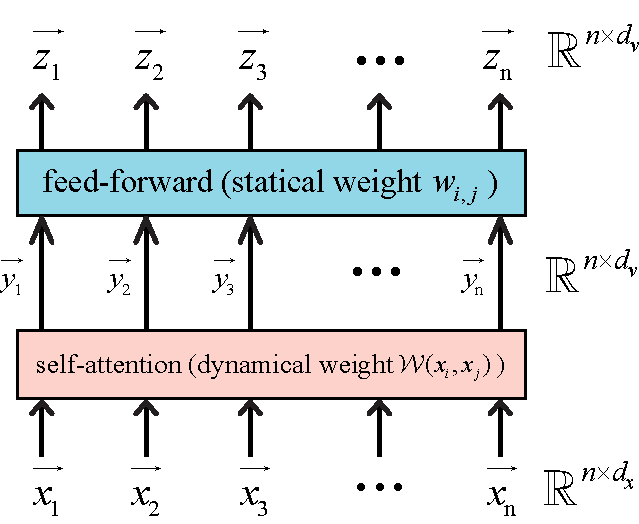
\includegraphics[width=0.9\linewidth]{images/transformer-overall.pdf}
   }
\end{center}
   \caption{Transformer block: self-attention and feed-forward. The residual connection are omitted for clearer view.
   }
\label{fig:transformerover}
\end{figure}

Transformer Block consists of two layers: self-attention and feed-forward layer. Both of them perform the weighted sum on the input.

The input is row vectors $x_i$, in which $i$ is the input position, and $d_x$ is the dimension of each input vector. There are total $n$ positions ($n$ word embeddings).

\begin{align*}
    x_i=[x_i^1, x_i^2, ..., x_i^{d_x}]\in\mathbb{R}^{1\times{d_x}}, i\in[1,n]
\end{align*}

Self-attention layer can be modeled generally as \autoref{eq:all-sa}, and feed-forward as \autoref{eq:all-ff}. In \autoref{eq:all-sa}, $y_i$ is the output of self-attention layer, and in \autoref{eq:all-ff} $z_i$ is the output of whole transformer block, as shown in \autoref{fig:transformerover}. the $y_i, z_i\in\mathbb{R}^{1\times{d_v}}$, $i\in[1,n]$. $\mathbb{N}$ is the normalization operation. $\mathcal{W}(x_i,x_j)$ is the self-attention value between input position $i$ and $j$. 

\begin{align}
    {y_i}&=\mathbb{N}\left[\sum_{j}\mathcal{W}(x_i,x_j)\times{v}({x_j})+x_i\right]\label{eq:all-sa}\\
    {z_i}&=\mathbb{N}\left[\sum_jw_{i,j}\times{y_j}+y_i\right]\label{eq:all-ff}
\end{align}

\subsection{Specific Matrix Form in Attention Paper}
\label{sec:spe}
\autoref{eq:all-sa} gives a general representation of transformer. Specifically, by the definition from~\cite{vaswani2017attention}, the $\mathcal{W}(x_i,x_j)=Softmax(\frac{\langle x_iW^q,x_jW^k\rangle}{\sqrt{d_k}})$, and $v(x_j)=x_jW^v$. The $W^q, W^k, W^v$ are weight matrix to be train. $W^q,W^k\in\mathbb{R}^{{d_x}\times{d_k}}$, $W^v\in\mathbb{R}^{d_x\times{d_v}}$.

If define $X=[x_1;x_2;...;x_n]$\footnote{Symbol ; means $X$ is column vector of $x_i$. $X$ is the input matrix containing all $n$ positions.}, $Y=[y_1;y_2;...;y_n]$, we have:

\begin{align}
    Y&=\mathbb{N}\left[Softmax\left(\frac{XW^q(XW^k)^T}{\sqrt{d_k}}\right)XW^v+X\right]\\
     &=\mathbb{N}\left[Softmax\left(\frac{XW^q(W^k)^TX^T}{\sqrt{d_k}}\right)XW^v+X\right]
\end{align}

Let $Q=XW^q, K=XW^k, V=XW^v$, than $Q,K\in\mathbb{R}^{n\times{d_k}}$, $V\in\mathbb{R}^{n\times{d_v}}$. We have self-attention layer defined as \autoref{eq:attn}. It is the same formula given in~\cite{vaswani2017attention}.

\begin{equation}
    Y=\mathbb{N}\left[Softmax\left(\frac{QK^T}{\sqrt{d_k}}\right)V+X\right]\label{eq:attn}
\end{equation}
    

\subsection{Scale-invariant Mapping}
\label{sec:simap}

All the input of self-attention layer are mapped to a higher dimension space\footnote{$Q,K,V$ follow the definition in~\cite{vaswani2017attention}}:

\begin{align}
    Q=XW^q,K=XW^k: \mathbb{R}^{n\times{d_x}}&\to\mathbb{R}^{n\times{d_k}}\\
    V=XW^v: \mathbb{R}^{n\times{d_x}}&\to\mathbb{R}^{n\times{d_v}}
\end{align}

This mapping has two important features:

\begin{enumerate}
    \item Invariant in scale. $X\to Q,K,V$ are scale-invariant mapping, which means for all the vectors $x_i$, the mapping operations $W^{q}$ are the same, and the relative position between $i$-th vector and $j$-th vector won't change. E.g. $q_1=x_1W^q, q_2=x_2W^q$, with $W^q$ shared, $q_1, q_2$ will follow the same distribution as $x_1, x_2$.
    \item Inherited chain. E.g. $q_i\sim x_i$ and only related with $x_i$. Or in other words, $q_i$ is a direct and exclusive projection of $x_i$. The mapping can be inherited to form a long chain. E.g. given $Q=XW^q, E=QW^e, F=EW^f$, we still have $f_1\sim e_1\sim q_1\sim x_1$.
\end{enumerate}

We can treat $Q,K,V$ as $X$ in the following analysis with the above two properties.

\textbf{Is it necessary to re-scale the $d_x$ input to $d_v$ output?}
As shown in \autoref{sec:statisapp}, the longer the intermediate dimension is, the more accurate that inner-product could estimate the attention.


\subsection{Deconstruct Self-attention}
\label{sec:self-attn}

As proved in \autoref{sec:simap}, mapping $Q=XW^q: \mathbb{R}^{n\times d_x}\to\mathbb{R}^{n\times d_k}$ is a scale-invariant mapping, similar for $V,K$. Thus we could replace $Q,K,V$ with $X$ in \autoref{eq:attn} to see what self-attention layer does to $X$:

\begin{equation}
    Y\sim \mathbb{N}\left[Softmax\left(\frac{XX^T}{\sqrt{d_k}}\right)X+X\right]
\end{equation}

Knowing $Softmax(\cdot)$, $(\frac{\cdot}{\sqrt{d_k}})$ and $\mathbb{N}[\cdot]$ are statistical operations, we can also remove them to have a clear view to the self-attention:

\begin{equation}
    Y\sim XX^TX+X\footnote{What if $Y\sim Q\times Softmax\left(\frac{K^TV}{\sqrt{d_k}}\right)+X$?}\label{eq:attn-sim}
\end{equation}

\autoref{eq:attn-sim} is a concise model revealing the self-attention layer's intrinsic structure.

\subsection{Feed-forward}
\label{sec:ff}

For comparison with self-attention, feed-forward's simplified formula are given in \autoref{eq:ff-sim} (matrix version of \autoref{eq:all-ff}, $W \in \mathbb{R}^{n\times n}$ is a static weight matrix):

\begin{equation}
    Z\sim WY + Y\label{eq:ff-sim}
\end{equation}

\textbf{What is the difference between self-attention and feed-forward?}
Compare \autoref{eq:attn-sim} and \autoref{eq:ff-sim}. They are both weighted sum of input, but self-attention uses dynamic weight matrix $XX^T$, while feed-forward uses static one. For self-attention, weight $XX^T=\{\langle\vec{x_i},\vec{x_j}\rangle\}$ is the \textbf{inner-product} that measures the similarity between $x_i, x_j$\footnote{Does similar input vector means the two position should have stronger attention?: No}. While for feed-forward, weight $W=\{w_{i,j}\}$ is a fixed weight, measuring the contribution from each input $x_j$ to the output $y_i$.

\section{Statistical Approach}
\label{sec:statisapp}
As shown in \autoref{sec:ff}, self-attention outperforms feed-forward by using a inner-product in its weight matrix. It implicitly assumes that the inner-product could represent the intrinsic relationship between the two positions. 

However, as shown in \autoref{sec:ip}, the inner-product can not always hold a solid measure of the positions' relationship. The normalization parameter $\sqrt{d_k}$ is not reasonable as well.

Let us take a look from the statistical view. We can take input vectors as stochastic processes, as \autoref{sec:rp} shows. We could use cross-correlation to measure the relationship between two inputs. The significance of such analysis is to find out self-attention's essence and be clear about implicit assumptions, so people can make improvements solidly.

\subsection{Inner-product}
\label{sec:ip}

Whether inner-product stands for the intrinsic relationship depends on the design of word-embedding. For example, in sentence ``{\tt I am fat cat}", the word ``{\tt I}" should have high co-existence with ``{\tt am}". Let ``\texttt{I}" have word embedding $x_1$, and ``\texttt{am}" have word embedding $x_2$. If $x_1, x_2$ not designed properly, the inner-product $\langle x_1, x_2 \rangle$ could be very low. \autoref{fig:wordemb} shows an illustration when $d_x=2$.

\begin{figure}[ht]
\begin{center}
\fbox{
   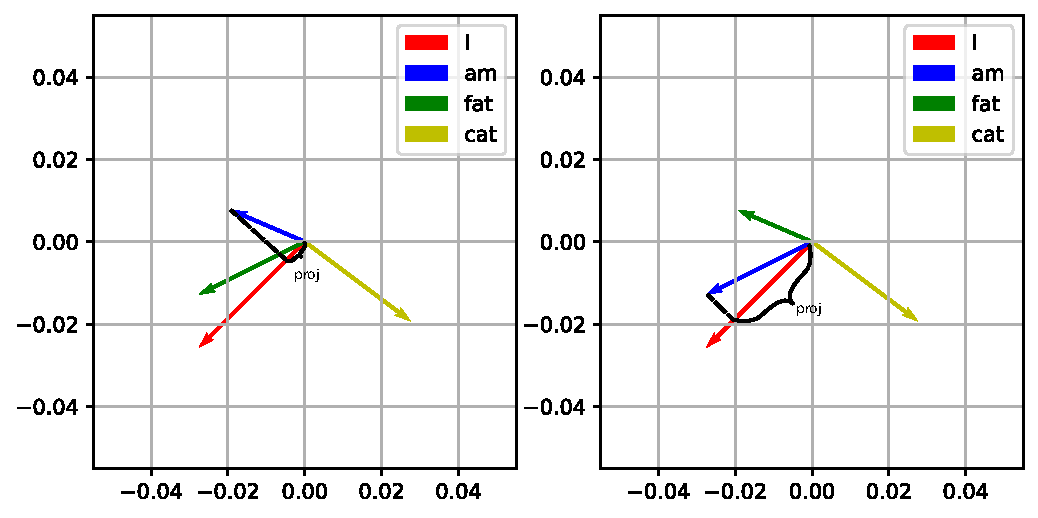
\includegraphics[width=0.9\linewidth]{images/word-embedding2.pdf}
   }
\end{center}
   \caption{Design of input vectors affects the projection greatly. In this case, the single inner-product can not reflect the strength of the relationship.
   }
\label{fig:wordemb}
\end{figure}


\subsection{Random Processing Model}
\label{sec:rp}

In probability theory, random processing $X$ is defined as an ensemble of all possible sample functions which describes the process' evolution through time~\cite{proakis2001digital}:

\begin{equation}
    X(t, S_x)
\end{equation}

in which $t$ is time, and $S_x$ is the sampling space of all possible sample functions. On time $t=t_1$, the $X(t_1, S_X)$ is a random variable. By the same definition, we have another random processing $Y(t,S_Y)$, as shown in \autoref{fig:randomp}

\begin{figure}[ht]
\begin{center}
\fbox{
   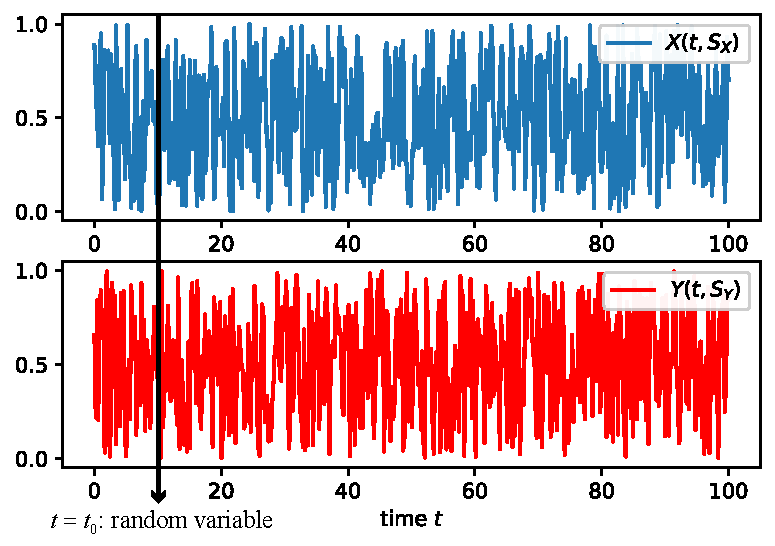
\includegraphics[width=0.9\linewidth]{images/randomprocess.pdf}
   }
\end{center}
   \caption{Random processing. At fixed time $t_0$, $X(t=t_0,S_X)$ is a random variable. Cross-correlation between random processing reveals the relationship between $S_X, S_Y$.
   }
\label{fig:randomp}
\end{figure}

Cross-correlation is a measure of two random processing's distribution correlation at time $t_1, t_2$:

\begin{equation}
    \gamma_{XY}(t_1,t_2)=E\left[X(t_1, S_X)Y(t_2, S_Y)\right]
\end{equation}

Based on above definition, we could model self-attention's input $x_i, x_j$ as two time samples of two random processing $X_i(t, S_{i}), X_j(t, S_{j})$ at same time $t=t_0$. Notice the two position $i,j$ have different sample space $S_i, S_j$:

\begin{align}
    x_i &= \left. X_i(t, S_i)\right\vert_{t=t_0}\label{eq:xi}\\
    x_j &= \left. X_j(t, S_j)\right\vert_{t=t_0}
\end{align}

$t_0$ is the sample time. For machine learning, $t$ means different batches of data.

Note that $x_i=\{x_i^{\alpha}\},\alpha\in[1,d_x]$ is not a value but a row vector of $1\times d_x$ dim. \textit{Assume each dimension of $x_i$ are i.i.d.\footnote{Independent and Identically Distributed} random variables in sampling space $S_i$}, we could treat each element $x_i^{\alpha}$ as a sample on time $t=t_0$, and we totally have $d_x$ samples. Similar for $x_j$.

\subsection{Cross-correlation}
\label{sec:cc}

Instead of treating the input as a static vector, we could model input as random processing with a different distribution, as shown in \autoref{eq:xi}.

Attention is human's recognition should be ``the tendency of two items have related changing." Intuitively, the correlation is a exact metric of this. 

The cross-correlation between random processing $X_i(t, S_i)$ and $X_j(t, S_j)$ is:

\begin{equation}
    \gamma_{ij}(t_1,t_2)=E[X_i(t_1, S_i)X_j(t_2, S_j)]
\end{equation}

Especially within same batch ($t_1=t_2=t_{batch}$), cross-correlation is average over $d_x$ samples:

\begin{align}
    \gamma_{ij}(t_{batch})&=E[X_i(t_{batch}, S_i)X_j(t_{batch}, S_j)] \\
                          &=\lim_{d_x\to\infty}\left(\frac{x_ix_j^T}{d_x}\right)\label{eq:true-cc}\\
                          &\approx\frac{x_ix_j^T}{d_x}\label{eq:sim-cc}
\end{align}

\autoref{eq:true-cc} gives a measure to correlation between two positions' distribution $S_i$ and $S_j$. Because infinite of samples are not possible, in practice people can use $d_x$ samples to estimate the real correlation, as shown in \autoref{eq:sim-cc}.

This explanation seems similar but is different from the inner-product one. By treating the input as random processing, we could know the good performance of the self-attention mechanism is based on static properties. Inner-product is a limited estimation to the cross-correlation. This also explains why need to do the mapping $\mathbb{R}^{n\times d_x} \to \mathbb{R}^{n\times d_v}$. The longer the $d_v$ is, the more sampling results we have, the more stable self-attention is.

{\small
\bibliographystyle{ieee_fullname}
\bibliography{ref}
}

\end{document}
